% Discription of what LSD-SLAM is, how it works and implementation

\chapter{LSD-SLAM\authorA}\label{ref:lsdslam}

\section{What is LSD-SLAM?}
LSD-SLAM stands for \textbf{L}arge-\textbf{S}cale \textbf{D}irect Monocular \gls{slam} and is a fairly new real-time monocular \gls{slam} that is fully direct-driven instead of relying on keypoint/keyfeature \cite{lsdslam_eccv}. The algorithm works on the image intensity for tracking and mapping at the same time.\newline
This method allows building large-scale maps on normal processors that are consistent when comparing it to current state-of-the-art algorithms. \newline
\begin{figure}[h]
	\centering
	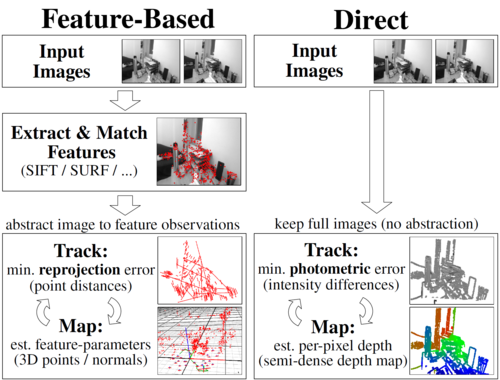
\includegraphics[height=0.5\textwidth]{./media/images/direct-vs-feature-based.png}
  	\caption{Feature-Based and Direct Difference
  	\\Src: \url{https://tinyurl.com/ycmjhb9d}}
  	\label{featurebased_direct_difference}
\end{figure}

\section{Difference Feature-Based and Direct}
\begin{itemize}
    \item \underline{Feature-based} \newline
        A feature-based \gls{slam} (e.g. ORB-SLAM \ref{ref:orbslam}) looks for distinctive points in the image and then uses only these keypoints to process the information. When there are only a few prominent keypoints (e.g indoor, tunnels) the result will not be that accurate.
    \item \underline{Direct} \newline
        Direct based \gls{slam}s use all information that's provided in the image. This does not only include distinctive points but also edges and sometimes surfaces and thus makes it possible to create a more accurate and denser 3D map \cite{lsdslam_eccv}.
\end{itemize}
\begin{figure}[h]
	\centering
	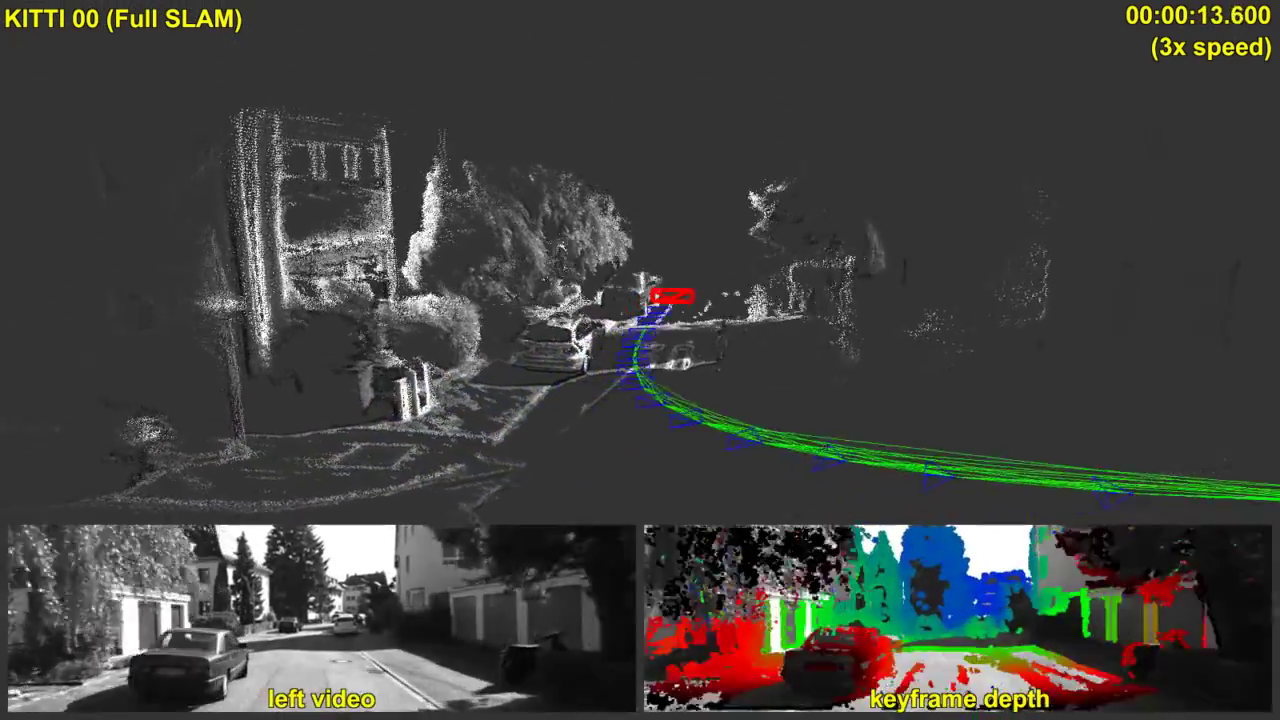
\includegraphics[width=0.7\textwidth]{./media/images/lsd-slam.png}
  	\caption{LSD-SLAM Example image
  	\\Src: \url{https://tinyurl.com/qkuamyy}}
  	\label{lsdslam}
\end{figure}

\section{How does the LSD-SLAM work?}
\subsection{Components that make up the LSD-SLAM}
\begin{itemize}
    \item \underline{Tracker} \newline
        The \textit{Tracking} component uses the current frame in relation to the last frame to continuously track the camera movement.
    \item \underline{Depth Map Estimation} \newline
        \textit{Depth map estimation} is done using tracked frames to refine or replace the current frame. Depth information is calculated by filtering over a small per-pixel baseline. If the camera has moved too far or the image has changed too much a new keyframe is initialized \cite{lsdslam_eccv}.
    \item \underline{Map Optimization} \newline
        When a keyframe gets replaced as a tracking reference, the refinement process stops and it gets included in the 3D depth map. \textit{Map optimization} then starts working to detect loop-closures or scale-drifts. This is done by a similarity transformation to frames that where taken nearby.
\end{itemize}

\subsection{Depth Map Estimation}
New keyframes are created when there where no frames before or the camera has moved/rotated so far that the set threshold has been exceeded. When this happens the new latest frame is chosen to become the new keyframe and the keypoints from the previous keyframe get projected onto the new one. The process is followed by scaling to fit the needs of the Direct Image Alignment. When that is done the keyframe replaces the previous ones and gets used to track the subsequent frames.\newline
Not every frame results in a new keyframe. Frames that don't make it to a new keyframe are used to improve and refine the current keyframe. The refinement is done by using a small stereo comparison for regions in an image where the expected use for advancement is higher. The result of this comparison gets merged into the existing 3D point cloud to add potentially new information or refining existing pixels \cite{lsdslam_eccv}.

\subsection{Map optimization}
Scaling, rotation and movement is not always perfect, which results in drift. Even if the drift effect is little it adds up, which might result in a very distorted map \cite{lsdslam_eccv}. The Pose-Graph-Optimization is an optimization algorithm which aims to fix these drifts with pretty good results. The advantages of the pose-graph-optimization are that it is fast and vulnerable for poor initialization estimates \cite{posegraphoptimization}. \newline

\begin{figure}[h]
	\centering
	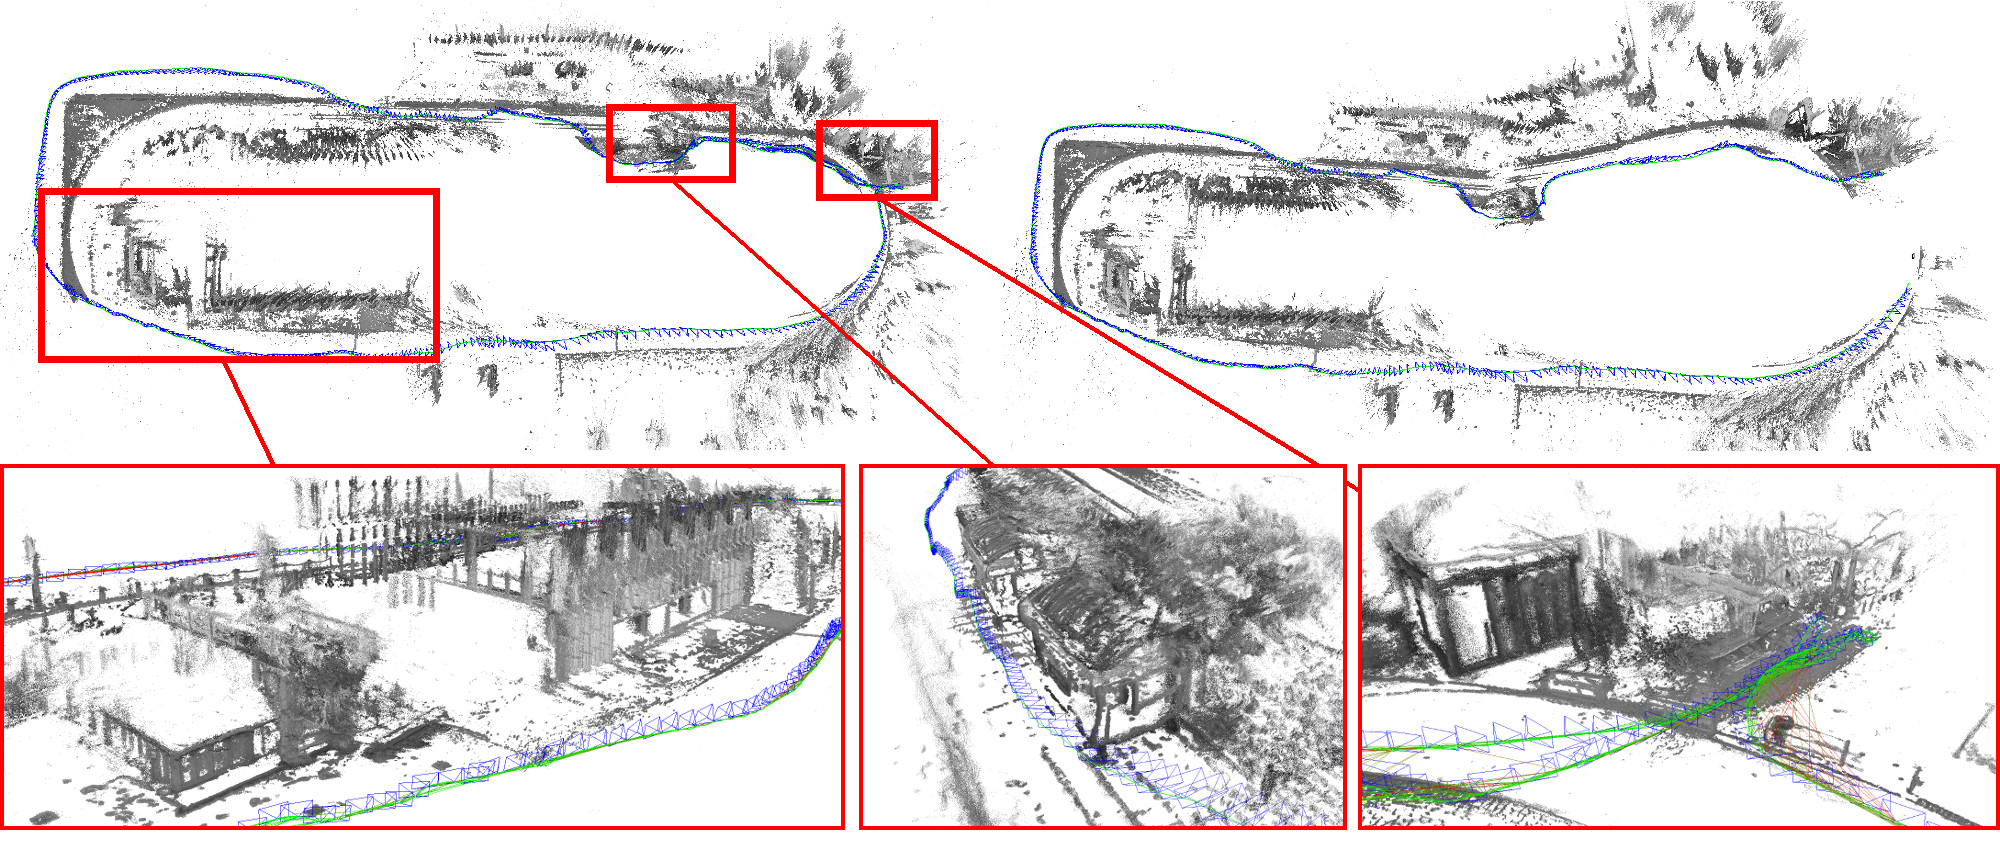
\includegraphics[width=0.8\textwidth]{./media/images/lsd-slam-pose-graph-optimization.jpg}
  	\caption{LSD-SLAM Pose-Graph-Optimization (left after loop-closure, right before loop-closure)
  	\\Src: \url{https://tinyurl.com/qkuamyy}}
  	\label{lsd-pose-graph-optimization}
\end{figure}

\subsection{Input/Output}
\textbf{Input Data:} rectified monocular image, camera info\\
\textbf{Output Data:} image with probability colored points, 3D point cloud